% \documentclass[aps,11pt,citeautoscript,reprint]{revtex4-1}
\documentclass[aps,twocolumn,10pt,reprint]{revtex4}
\usepackage[export]{adjustbox}
\usepackage{geometry}
\geometry{
a4paper,
 total={170mm,257mm},
 left=15mm,
 right=15mm,
 top=15mm,
 bottom=15mm,
}
\usepackage{graphicx}
\usepackage{epsfig}
\usepackage{amsmath}
\usepackage{graphicx}% Include figure files
\usepackage{dcolumn}% Align table columns on decimal point
\usepackage{bm}% bold math
\usepackage{amssymb}
\usepackage{amsmath}
\usepackage{epsf}
\usepackage{subfigure}
\usepackage{epstopdf}
\usepackage{color}
\usepackage{array}
\usepackage{subeqnarray}
\usepackage{mathrsfs}
\usepackage{float}
\usepackage[colorlinks=true, pdfstartview=FitV, linkcolor=red, citecolor=blue, urlcolor=blue]{hyperref}
\usepackage[font=fontsize]{caption}



% \newcommand\huge{\@setfontsize\huge\@xxpt{25}}
\newcommand{\be}{\begin{equation}}
\newcommand{\ee}{\end{equation}}
\newcommand{\ben}{\begin{eqnarray}}
\newcommand{\een}{\end{eqnarray}}

\makeatletter
\renewcommand{\fnum@figure}{\it{Figure} \thefigure}
\makeatother

\renewcommand{\thefootnote}{\roman{footnote}}

\begin{document}

\title{Set 5 - Modelling data with power laws (Pareto’s law and Zipf’s law)}

\author{Yash Kodwani [202101418]}\email{202101418@daiict.ac.in}
\affiliation{Dhirubhai Ambani Institute of Information \& Communication Technology, Gandhinagar, Gujarat 382007, India\\ CS302, Modeling and Simulation}
\author{Bhavya Shah [202101426]}\email{202101426@daiict.ac.in}
\affiliation{Dhirubhai Ambani Institute of Information \& Communication Technology, Gandhinagar, Gujarat 382007, India\\ CS302, Modeling and Simulation}

% abstract should mention what is done in the lab and the key observation 
\begin{abstract}

\textbf In this lab we modelled the Pareto
distribution of wealth in India.
\end{abstract}



\maketitle


\section{PARETO'S LAW}

Pareto's Power Law, also known as the Pareto Distribution, is a statistical concept that describes the distribution of wealth, income, and other quantities in many real-world situations. Given that x is the amount of wealth and N(x) is the frequency distribution of wealth holders,
\\
\be\label{Eq:Logisticeq}
N(x) = A+Bx^{-\alpha}
\ee
\\
\subsection{Plot $N(x)$ versus x}
\vspace{-5mm}
\begin{figure}[!h]
    \centering
    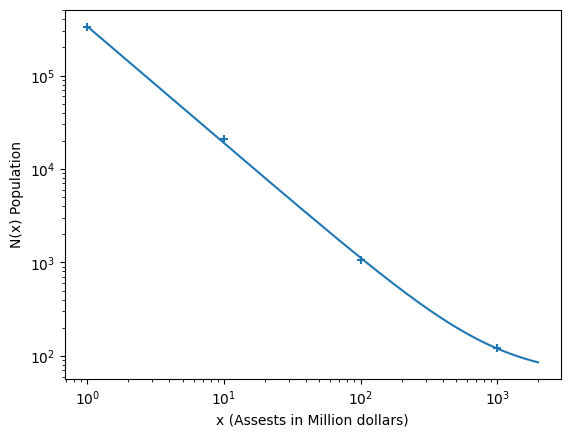
\includegraphics[width=1\linewidth, center]{images/lab4_cs_1.png}
    \vspace{-5mm}
    \caption{The plot of N(x) vs x, A = 60, B=336000, $\alpha=5/4$}
    \label{fig:q1_1}
\end{figure}

\newpage
\section{ZIPF'S LAW}
In the context of the dependency network of Debian, Zipf's law would imply that there is
 a power-law relationship between the frequency of dependencies and their rank.
 In other words, a small number of packages would have a high frequency of dependencies,
  while a large number of packages would have very few dependencies.
This is the differential equation for continuum model for any power-law feature,
\be\label{Eq:firstEquation}
(x+ \lambda) \dfrac{d\phi}{d\x} = \alpha \phi (1 - \eta \phi ^ {\mu})
\ee
where, $ \alpha$ is a power-law exponent, $\mu$ is a nonlinear saturation exponent, $\eta $ is a tuning parameter and $\lambda$ is another parameter for instrumental in setting a limiting scale for poorly connected node
\newline

\noindent Integrating this \eqref{Eq:firstEquation} gives
\be\label{Eq:single-dose-x}
\phi(x) =   [\eta + (\dfrac{x+\lambda}{c})^{- \mu \alpha}]^{-1/\mu}]
\ee
With $\mu = -1$ and with $\alpha = -2$ (Zipf's Law)   
\be\label{Eq:single-dose-x}
\phi(x) =   \eta + (\dfrac{c}{x+\lambda})^{2}
\ee

\subsection{Plot of $\phi(x)$ versus x for Etch Release }
    
    \begin{figure}[H]
        \centering
        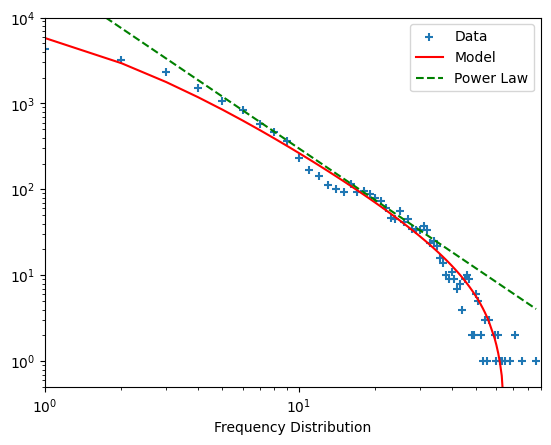
\includegraphics[width=1.0\linewidth, center]{images/lab5_q2_1.png}
        \vspace{-2mm}
        \caption{For the network of incoming links in the Etch release, degree distribution shows a good fit for $\alpha=-2$, $\eta=-8$, $\lambda=-1.5$, $\mu = -1$ and $c =190$ }
        \label{fig:q2}
    \end{figure}
    
    \begin{figure}[H]
        \centering
        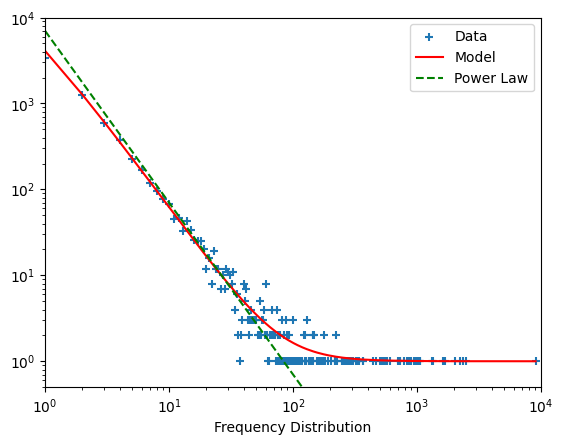
\includegraphics[width=1.0\linewidth, center]{images/lab5_q2_2.png}
        \vspace{-2mm}
        \caption{For the network of outgoing links in the Etch release, degree distribution shows a good fit for $\alpha=-2$, $\eta=1$, $\lambda=0.25$, $\mu = -1$ and $c =80$}
        \label{fig:q2}
    \end{figure}

\vspace{-5mm}    
\subsection{Plot of $\phi(x)$ versus x for Denny Release }
\vspace{-5mm}
    \begin{figure}[H]
        \centering
        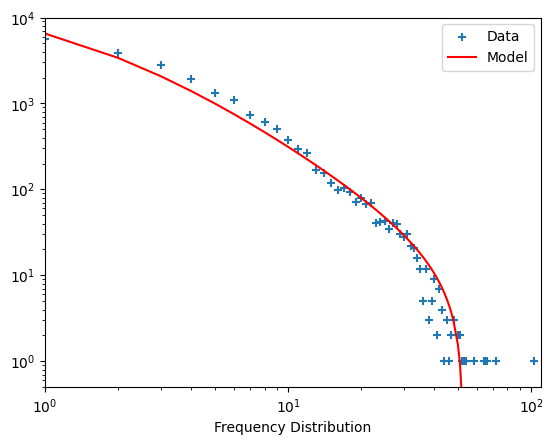
\includegraphics[width=1.0\linewidth, center]{images/lab5_q2_3.png}
        \vspace{-2mm}
        \caption{For the network of incoming links in the Denny release, degree distribution shows a good fit for $\alpha=-2$, $\eta=-15$, $\lambda=1.6$, $\mu = -1$ and $c =210$ }
    \end{figure}
\begin{figure}[H]
        \centering
        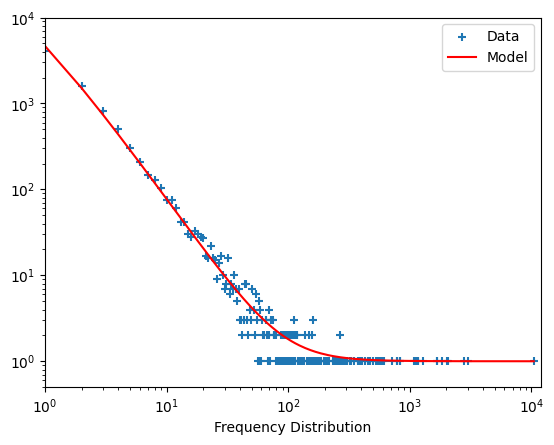
\includegraphics[width=1.0\linewidth, center]{images/lab5_q2_4.png}
        \vspace{-2mm}
        \caption{For the network of outgoing links in the Denny release, degree distribution shows a good fit for $\alpha=-2$, $\eta=1$, $\lambda=0.35$, $\mu = -1$ and $c =90$ }
        \label{fig:q2}
    \end{figure}

\subsection{Plot of $\phi(x)$ versus x for Squeeze Release }

    \begin{figure}[H]
        \centering
        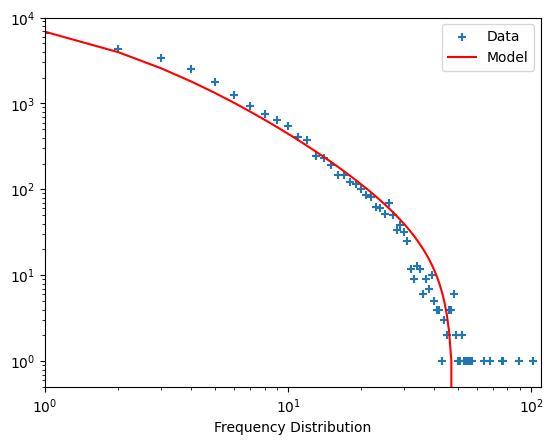
\includegraphics[width=1.0\linewidth, center]{images/lab5_q2_5.png}
        \vspace{-2mm}
        \caption{For the network of incoming links in the Squeeze release, degree distribution shows a good fit for $\alpha=-2$, $\eta=-28$, $\lambda=2.2$, $\mu = -1$ and $c =265$ }
        \label{fig:q2}
    \end{figure}

    \begin{figure}[H]
        \centering
        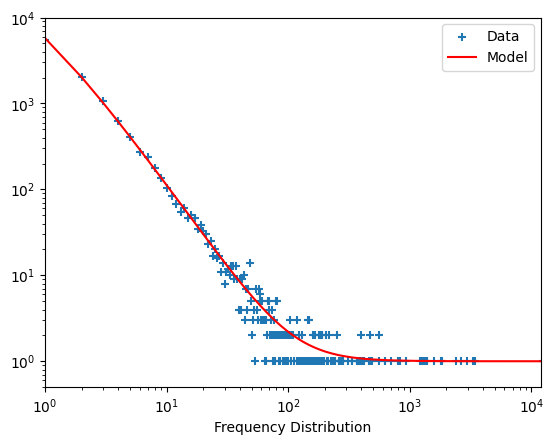
\includegraphics[width=1.0\linewidth, center]{images/lab5_q2_6.png}
        \vspace{-2mm}
        \caption{For the network of outgoing links in the Denny release, degree distribution shows a good fit for $\alpha=-2$, $\eta=1$, $\lambda=0.45$, $\mu = -1$ and $c =110$ }
        \label{fig:q2}
    \end{figure}

\section{Conclusion}

\begin{itemize}
    \item   In economic models and simulations, income and wealth distribution are often modeled using Pareto distributions. This distribution suggests that a small percentage of the population holds the majority of wealth, while the majority of people have relatively little wealth.
\vspace{-5mm}
    \item
    The mathematical model developed for analyzing the Debian GNU/Linux network quantitatively distinguishes between incoming and outgoing distributions, allowing for the study of saturation properties and directional characteristics
    \vspace{-5mm}
    \item The parameter A in the pareto's law show the saturation amount 
\end{itemize}

\end{document}